\documentclass[11pt]{article}
\usepackage[margin=1in]{geometry}
\usepackage{graphicx}
\usepackage{float}
\usepackage{amsmath}
\usepackage{amssymb}
\usepackage{amsthm}
\DeclareMathOperator*{\argmin}{argmin}
\DeclareMathOperator*{\argmax}{argmax}
\newtheoremstyle{ModifiedStyle}
{\topsep} % Space above
{3pt} % Space below
{} % Body font
{} % Indent amount
{\bfseries} % Theorem head font
{.} % Punctuation after theorem head
{.5em} % Space after theorem head
{} % Theorem head spec (can be left empty, meaning 'normal')
\theoremstyle{ModifiedStyle}
\theoremstyle{ModifiedStyle}
\newtheorem{remark}{Remark}
\usepackage[
    backend=biber,
    style=authoryear,
  ]{biblatex}

\addbibresource{main.bib}

\title{Simulation Study Overview}
% \author{Jose I. Velarde Morales}

\begin{document}
\maketitle
\tableofcontents

% \section{Introduction}
%   One of the chief criticisms of the US criminal justice system is that many states in the US have large regional variation in sentencing. This means that given the same crime, the probability of incarceration and the length of sentence varies considerably from county to county. To reduce variability in sentencing, many states (e.g. Florida, Minnesota, Washington) have introduced sentencing guidelines. These guidelines generally reduce the amount of discretion a judge has when deciding the length of a sentence. \cite{hester2012criminal} found that South Carolina has less county-level variation in sentencing than many states with sentencing guidelines.
%
%   A follow up study (\cite{hester2017conditional}) suggests that this might be due to the practice of judge rotation in South Carolina.
%   Judges in South Carolina don't sit exclusively in one county. Instead, they split their time amongst several counties in the state. For reference, the average judge hears cases in 12 counties throughout the year. Defendants are given some choice with regards to the date their case will be heard. Furthermore, defendants are made aware of which judges will be sitting in which counties in the near future. This gives them the ability to "shop" for judges, although subject to some constraints (e.g. judge availability).
%
%   The goal of this project is study how some system features affect sentencing outcomes. The system features we focus on are judge capacity and defendant choice. The outcomes we focus on are across county variation in sentencing and backlog of defendants. We study the system through simulation. We estimate relevant parameters using a rich dataset of sentencing data from South Carolina. The model we simulate builds on the work of \cite{wang2019}.

\section{Data}
  We have two main data sources: sentencing data and judge schedules, both of them are for the 2001 fiscal year. We obtained the data from the authors of \cite{hester2017conditional}. We briefly describe both datasets below.

  \subsection{Sentencing Data}
    The sentencing data contains information about 17,671 sentencing events in South Carolina from August 2000-July 2001. Each sentencing event contains an identifier for the judge who heard the case, the county the case was heard in, categorical variables describing the offense, and some defendant characteristics (e.g. race, age, and criminal history). There are 50 judges and 46 counties in the dataset. A full list of the variables can be found in table \ref{sent-vars}.
    \begin{table}[H]
      \caption{Sentencing Data Variables}
      \label{sent-vars}
      \begin{tabular}{|l|l|}
\hline
\textbf{Variable} & \textbf{Description}                                             \\ \hline
date              & date of sentence                                                 \\ \hline
county            & county where the sentence was decided                            \\ \hline
circuit           & circuit court where sentence was decided                         \\ \hline
judge             & numerical identifier for the judge who head the case             \\ \hline
trial             & binary variable indicating whether the case went to trial        \\ \hline
incarc         & binary variable indicating whether the sentence includes incarceration                \\ \hline
statute           & the code of law that the offender broke (e.g. 56-05-0750(B)(1))  \\ \hline
offdescr          & a description of the offense (e.g. driving under the influence)  \\ \hline
counts            & numerical variable                                               \\ \hline
statute\_first & the code of law that the offender broke, identical to 'statute' variable              \\ \hline
offdescr\_first   & a description of the first offense, similar to offdescr          \\ \hline
offtyped       & detailed categorical offense type, there are 10 values (rape, assault,   theft, etc). \\ \hline
sgc\_offcode   & a numerical code that is used to determine the minimum sentence   multiplier          \\ \hline
offtypeLibHyp     & categorical offense type (property, violent, drug, other)        \\ \hline
offser            & offense seriousness, ranges from 1-8                             \\ \hline
ccpnts            & numeric values between 1 and 68                                  \\ \hline
ccpts99           & commitment score, an alternative measure of offense seriousness. \\ \hline
crimhist          & defendant criminal history, takes 5 categorical values           \\ \hline
ppoints           & numerical values between 0-1014                                  \\ \hline
male              & binary variable indicating sex                                   \\ \hline
age               & age of defendant at sentencing, ranges 15-81                     \\ \hline
black             & binary variable indicating whether defendant is black            \\ \hline
sentence          & length of sentence in months, ranges 0-11988                     \\ \hline
expmin            & expected minimum sentence                                        \\ \hline
\end{tabular}

    \end{table}

    \subsubsection{Sample}
      In the raw data, there are 51 distinct judge ID's. However, according to \cite{hester2017conditional}, judge 1 is a combination of several judges that had few sentencing events. As a result, we exclude judge 1 from our sample, which leaves us with 17,516 observations.

  \subsection{Judge Schedule Data}
    This dataset contains information about each judge's assignment for each week of the fiscal year 2001. A snapshot of the calendar can be seen in figure \ref{fig-calendar}. Each assignment generally contains the county each judge was assigned to and the assignment type. The assignment type refers to the kind of cases a judge is scheduled to hear (civil or criminal).
    \begin{figure}[h]
        \centering
        \caption{Snapshot of Judge Calendar}
        \label{fig-calendar}
        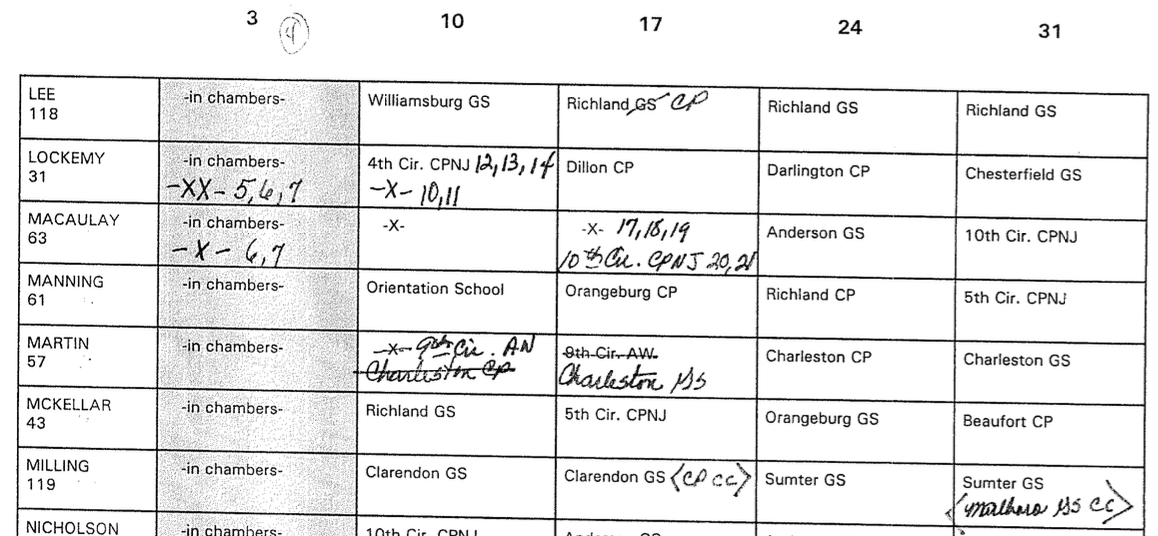
\includegraphics[width=0.75\textwidth, keepaspectratio=true]{Figures/Fig4.png}
      \end{figure}

    \subsubsection{Parsing}
      As can be seen from figure \ref{fig-calendar}, the assignments are on a weekly basis. A judge can be assigned to one or multiple counties in a week, and we observe 5 different kinds of assignments: single assignment, single assignment with dates, multiple assignment, multiple assignment with some dates, and multiple assignment with all dates. We parse the calendar data to determine each judge's schedule for every day of the year. In the resulting data, the unit of observation is judge, day, county. Note that the only potentially ambiguous assignment types are multiple assignment and multiple assignment with some dates. For these assignment types, we set the judge to be in all counties that he is scheduled to be in. For example, if judge 2 is scheduled for both Marion and Horry in the week of March 19-March 23, for each day of that week our data would include an observation for judge 2 in Horry and an observation for judge 2 in Marion. An example of what our parsed data looks like can be seen in table \ref{tab-calendar-example}.

      \begin{table}[H]
        \centering
        \caption{Assignment Types}
        \label{tab-assignments}
        \begin{tabular}{|l|l|}
\hline
\textbf{Assignment} & \textbf{Example}                \\ \hline
Single              & Marion                          \\ \hline
Single with dates   & Marion 23, 24, 25               \\ \hline
Multiple            & Marion, Horry                   \\ \hline
Multiple some dates & Marion 23, 24, Horry            \\ \hline
Multiple all dates  & Marion 23, 24, Horry 25, 26, 27 \\ \hline
\end{tabular}

      \end{table}

      \begin{table}[H]
        \centering
        \caption{Example of Parsed Calendar Data, here Judge 3 is scheduled for both Horry and Greenville on March 19.}
        \label{tab-calendar-example}
        
\begin{tabular}{|l|l|l|l|}
\hline
\textbf{Judge} & \textbf{Day} & \textbf{County} & \textbf{Days Assigned} \\ \hline
2              & 2001-03-19   & Marion          & 1 \\ \hline
3              & 2001-03-19   & Horry           & 0.5 \\ \hline
3              & 2001-03-19   & Greenville      & 0.5\\ \hline
\end{tabular}

      \end{table}

    \subsubsection{Assignment Types}
      Judge calendar assignments generally have an acronym indicating the type of the assignment (e.g. Marion GS). There are eight different assignment types, each with a corresponding acronym. Assignments can have more than one type (e.g. Marion GS CC). Our study focuses on criminal cases, which are heard in general sessions (GS). Some assignment types, like CP (common pleas), are for civil cases. A full list of the assignment type acronyms and their meanings can be found in table \ref{tab-assignment-types}.

      \begin{table}[H]
        \centering
        \caption{Assignment Type Acronyms}
        \label{tab-assignment-types}
        \begin{tabular}{L{20mm}L{50mm}L{20mm}}
  \hline
  Acronym & Meaning & Share \\
  \hline
  %\rowgroup{Consumer Surplus} \\
  GS & General Session & 0.36 \\
  CC & Circuit Court & 0.02\\
  SGJ & State Grand Jury & 0.01\\
  CP & Common Pleas & 0.26 \\
  CPNJ & Common Pleas Non-Jury & 0.13 \\
  PCR & Post Conviction Relief & 0.03  \\
  Capital PCR & Capital Post Conviction Relief & < 0.01 \\
  AW & Administrative Week & 0.01 \\
  \hline
\end{tabular}

      \end{table}

\section{Model}
  We use the model developed by \cite{wang2019}. There are three agents: the judge, the defendant, and the prosecutor. The prosecutor proposes a plea offer, and the judge and the defendant choose whether to accept. The game evolves in the following steps:

  \begin{enumerate}
    \item The defendant chooses the judge/decides when to go to court
    \item The prosecutor makes a plea offer
    \item The defendant decides whether to accept the plea offer or go to trial
  \end{enumerate}

  Each defendant is characterized by the following quantities: $\theta$ - the probability of conviction at trial, and $\tau$ - the expected sentence length if convicted in trial. Each defendant additionally has an idiosyncratic cost of going to trial, $c_d >0$. A defendant will accept a plea offer, $s$, if $s \leq \theta \tau + c_d$.\\

  Judges are modeled by their harshness, $h$. Given a defendant, $\theta \tau$ and a plea offer, $s$, the lowest plea offer the judge will accept is denoted by $l_j(\theta \tau)$ and the maximum plea offer the judge will accept is denoted by $u_j(\theta \tau)$.\\

  As a result, given a specific judge $j$, the optimal sentence for the prosecutor to offer is $s^* = \min(\theta \tau + c_d,u_j(\theta \tau))$. This quantity is also the defendant's cost.

\section{Estimation}
  For the simulation, we have to estimate several of the model's parameters. In this section, we provide a detailed description of how we estimate each parameter, including the sample used.

  \subsection{Probability of Conviction at Trial - $\theta$}
    We currently estimate this using $l_2$ regularized logistic regression with a penalty parameter of 1. We use the following variables to predict this quantity: Black, Offense Type, and Offense Seriousness. We represent all variables as binary variables. We split our sample into train and test sets using a 75/25 split to evaluate the performance of our classifier. Our classifier's performance can be seen in table \ref{classifier-performance}. The classifier outputs prediction probabilities, which is what we use for $\theta$. The classifier's prediction probability can be interpreted as the probability that the observation will have a value of 1 for the incarceration variable. The final classifier we use to predict $\theta$ for all observations in our dataset is trained on the full training set.

    \begin{table}[H]
      \centering
      \caption{Evaluation Metrics for Classifier}
      \label{classifier-performance}
      \begin{tabular}{|l|l|}
      \hline
      \textbf{Metric} & \textbf{Score} \\ \hline
      AUC             & 0.93           \\ \hline
      F1              & 0.94           \\ \hline
      Accuracy        & 0.89           \\ \hline
      \end{tabular}
    \end{table}

    \subsubsection{Sample}
      We only use the observations in the data that are trials and that have non missing values for the predictor variables. There are only 256 observations in the data meeting this criteria.

    \subsubsection{Proposed Changes}
      We should consider jointly estimating $\theta$ and $\tau$ using a Hurdle Regression model as in Hester and Hartman 2017.

  \subsection{Expected Sentence Length if Convicted - $\tau$}
    We currently estimate this using Negative Binomial Regression. We use the Cameron-Trivedi test for overdispersion to choose the overdispersion parameter. As in Hester and Hartman 2017, our dependent variable is the expected minimum sentence. We use the following variables to predict this quantity: Black, Age, Offense Type, and Offense Seriousness.

    \subsubsection{Sample}
      We only use the observations in the data that are trials and that have non missing values for the predictor variables. There are only 256 observations in the data meeting this criteria.

    \subsubsection{Proposed Changes}
      We should consider jointly estimating $\theta$ and $\tau$ using a Hurdle Regression model as in Hester and Hartman 2017.

  \subsection{Defendant Cost of Trial - $c_d$}
    We are currently estimating this using only the first method described in the Write-Up. In this method, we use the subset of cases where the sentence, $s$, is less than $u_j(\theta \tau)$. In these cases, our model implies that $c_d = s - \theta \tau$.

    \subsubsection{Proposed Changes}
      We should implement the maximum likelihood estimation procedure described in Nasser's document for the other cases. Here's the discussion:
      Recall that $i=1,\ldots,I_j$ are the plea bargains judge $j$ oversaw, and that their sentence is given by $s_i=\min(\theta_i\tau_i+c_d(i),u_i)$, where $u_i = u_j(\theta_i\tau_i)$ and $u_j(\cdot)$ is defined above. We define the sets $\mathcal{I}_j^1$ and $\mathcal{I}_j^2$ as follows:
  			\begin{align*}
  				\mathcal{I}_j^1 &\,=\, \{i=1,\ldots,I_j: s < u_i\}, \\
  				\mathcal{I}_j^2 &\,=\, \{1,\ldots,I_j\} \,\backslash\, \mathcal{I}_j^1 \,=\, \{i=1,\ldots,I_j:s_i=u_i\}.
  			\end{align*}
  			Then, we can infer $c_d(i) = s_i - \hat{\theta}_i\hat{\tau}_i$ for $i\in\mathcal{I}_j^1$. On the other hand, we can only infer that $c_d(i) \geq u_i - \hat{\theta}_i\hat{\tau}_i$ for $i\in\mathcal{I}^2_j$.

  		Next, we let $K_j$ denote the number of trials judge $j$ oversaw, which are indexed by $k \in \mathcal{K}_j = \{1,\ldots,K_j\}$. Recall that a case goes to trial if $\theta_i\tau_i+c_d(i)<l_i$. Thus, for $i=1,\ldots,K_j$, we infer that $c_d(i) < l_i-\hat{\theta}_i\hat{\tau}_i$.

  		In summary, although we can impute $c_d(i)$ exactly for $i\in\mathcal{I}_j^1$, we can only infer that $c_d(i)$ falls into an interval for $i\in\mathcal{I}^2_j\cup \mathcal{K}_j$. However, assuming a parametric distribution for $c_d$, e.g., $c_d \sim N(\mu,\sigma^2)$, we can estimate its parameters using maximum likelihood. To this end, we let $F$ and $f$ denote the cdf and pdf of the distribution of $c_d$, and define the likelihood function $\mathscr{L}_j$ as follows:
  		\begin{align*}
  			\mathscr{L}_j \,=\, \prod_{i\in\mathcal{I}_j^1} f(s_i-\hat{\theta}_i\hat{\tau}_i) \prod_{i\in\mathcal{I}_j^2} \bar{F}(u_i-\hat{\theta}_i\hat{\tau}_i) \prod_{i\in \mathcal{K}_j} F(l_i-\hat{\theta}_i\hat{\tau}_i).
  		\end{align*}
  		Then, we let $\mathscr{L} = \prod_{j=1}^J \mathscr{L}_j$ and $\argmax \mathscr{L}$ helps us choose the parameters of the distribution $F$.
  		\begin{remark}
  			Note that the approach proposed immediately above allows $c_d$ to be negative. We can attribute this to $c_d(i)$ being the cost of trial plus an idiosyncratic shock specific to defendant $i$, which encompasses all factors that are not captured explicitly in the model.
  		\end{remark}
  		\begin{remark}
  			We envision drawing defendant profiles (along with their cases) with replacement from the dataset at a particular weekly rate in our simulation study. As we do so, we can set $c_d = c_d(i)$ whenever we draw a defendant who falls into the set $\mathcal{I}_j^1$ for some judge $j$. Otherwise, we can consider the following two cases:
  			\begin{itemize}
  				\vspace{-2mm}
  				\item[] \hspace{-10mm}\textbf{Case i)} Defendant $i$ is in the set $\mathcal{I}_j^2$ for some judge $j$. Then, we draw $c_d(i)$ from the conditional distribution $F(x|x\geq u_j-\hat{\theta}_i\hat{\tau}_i)$.
  				\vspace{-2mm}
  				\item[] \hspace{-10mm}\textbf{Case ii)} Defendant $i$ is in the set $K_j$ for some judge $j$. Then, we draw $c_d(i)$ from the conditional distribution $F(x|x\leq l_j-\hat{\theta}_i\hat{\tau}_i)$.
  			\end{itemize}
  		\end{remark}

  \subsection{Judge maximum and minimum plea - $l_j(\theta \tau),u_j(\theta \tau)$}
    \paragraph{Mathematical Description} Recall that a key quantity for us is $\theta\tau$. Fix a judge, say judge $j$, and focus only on the pleas he sentenced. For each such case, we can calculate $\hat{\theta}\hat{\tau}$ using the estimates from the hurdle model described in Section (tbd). Suppose judge $j$ handled $I_j$ such cases, indexed by $i=1,\ldots,I_j$. Let $\mathcal{A}_j$ denote the convex hull of the origin $(0,0)$ and the points $(\hat{\theta}_i\hat{\tau}_i,s_i)$ for $i=1,\ldots,I_j$. Given the set $\mathcal{A}_j$, we impute $l_j(\cdot)$ and $u_j(\cdot)$ as functions of $\theta\tau$ as follows:
		\begin{align*}
			&l_j(\theta\tau) \,=\, \min\{y:(\theta\tau,y)\in\mathcal{A}_j \} \\
			&u_j(\theta\tau) \,=\, \max\{y:(\theta\tau,y)\in\mathcal{A}_j \}
		\end{align*}

     \paragraph{Implementation}
     Suppose we have the simplices of the convex hull for a specific judge, and that they are given as tuples of two points $((x_1,y_1),(x_2,y_2))$. Given a specific $\theta \tau$ we implement the convex hull approach by iterating over the simplices of the convex hull, and finding the two simplices on which $\theta \tau$ lies. In other words, we find the two line segments on the boundary of the convex hull whose domain includes $\theta \tau$. We then find the value of the convex hull boundary at $\theta \tau$ in each of these two line segments using linear interpolation. The largest (smallest) of these two values is $u_j (l_j)$. \textbf{Note:} we should think about what to do in cases where $\theta_1 \tau_1$ is not in the convex hull. Figure \ref{fig-convex-hull} contains an illustration:

    \begin{figure}[H]
      \centering
      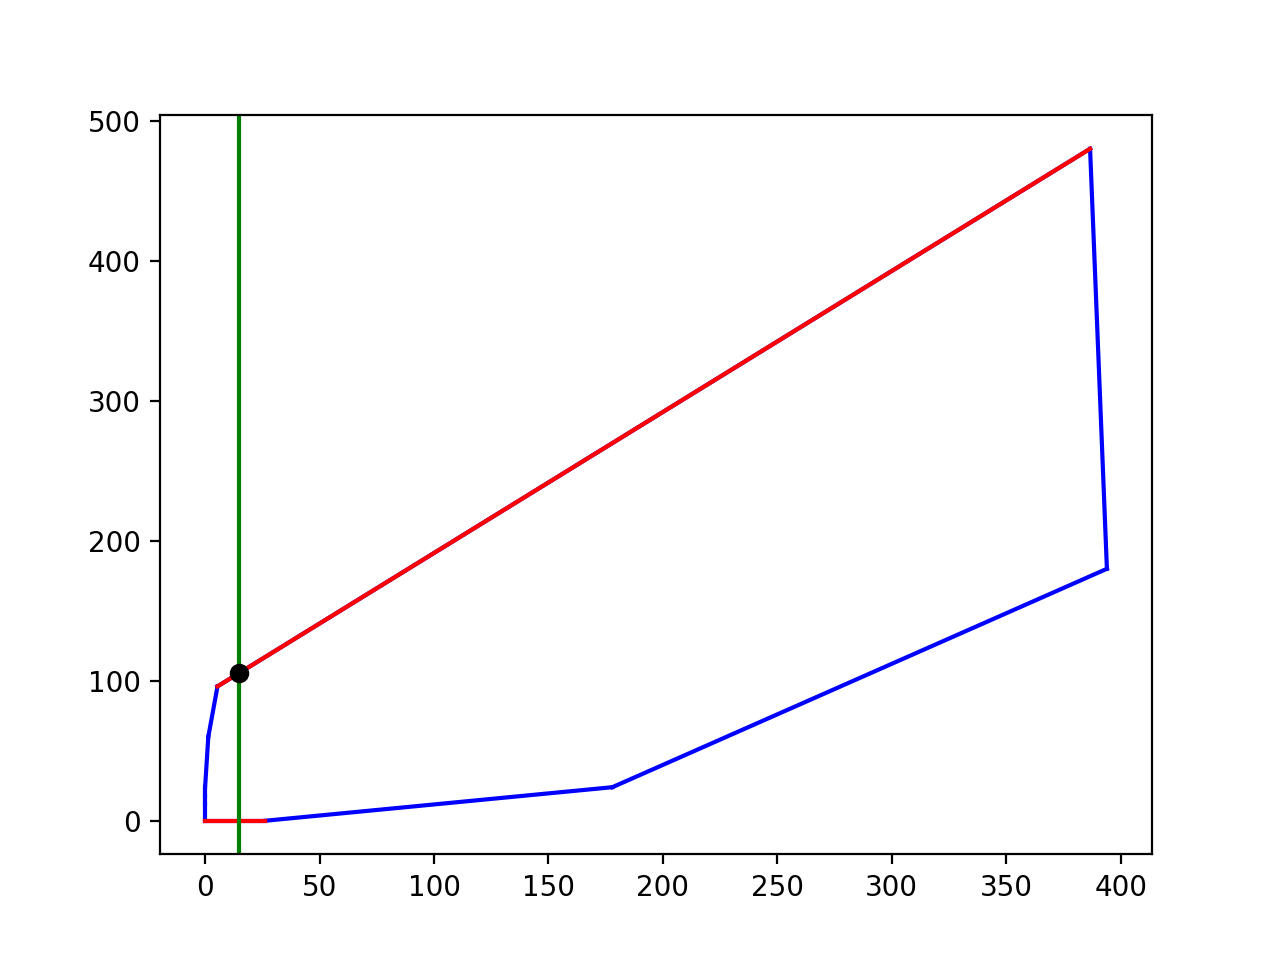
\includegraphics[width=0.65\textwidth]{../../output/figures/Exploration/convex_hull_max.png}
      \caption{Example of convex hull approach. The convex hull is in blue, the two line segments containing $\theta \tau$ are in red, and the green line intercepts the x-axis at $\theta \tau$. The black dot would be the maximum plea.}
      \label{fig-convex-hull}
    \end{figure}

    \subsubsection{Sample}
      Here, to estimate $l_j(\theta \tau),u_j(\theta \tau)$ for a specific judge, $j$, we use all of pleas judge $j$ heard. In other words, we exclude all of $j$'s trials. We also add the point $(0,0)$ to the convex hull of every judge.

  \subsection{County Arrival Rates - $\lambda_c$}
    We set each county's arrival rate to be equal to the average number of sentencing events per week in that county, as observed in the data. Let $N_{cw}$ denote the number of sentencing events in county $c$ in week $w$, county $c$'s arrival rate is defined as: $\lambda_c = \frac{\sum_w N_{cw}}{\sum_w 1}$. We are currently using all pleas and all weeks in our data to calculate this.

  \subsection{Service Rates - $\mu_p,\mu_t$}
    \subsubsection{Samples}
      \paragraph{Plea MLE Sample} This is the sample we use for the maximum likelihood estimation part of the ad-hoc algorithm. We also refer to this sample as "clean days". For this, we only consider pleas that happened on days which satisfy the following conditions:
        \begin{table}[H]
          \centering
          \caption{MLE Plea Sample Exclusion Criteria}
          \begin{tabular}{|l|}
          \hline
          \textbf{Condition}                                                  \\ \hline
          No inconsistencies between sentencing data and calendar \\ \hline
          Judge has at least 10 'clean' days                      \\ \hline
          Judge has at least one sentencing event that day         \\ \hline
          Judge is only assigned to one county that day          \\ \hline
          Judge only sentences in one county that day             \\ \hline
          Judge never has more than 35 sentencing events in this county \\ \hline
          Judge calendar assignment is of type "GS"           \\ \hline
          \end{tabular}
        \end{table}
      % \textbf{Sensitivity Analysis:} Add these one by one, similar to how controls are presented in Econ papers, and see how the quantity of interest changes as they are added. We could also add them in groups. Some of these correspond to outlier control and others to day cleanliness. We can run it with and without each group.

      \paragraph{Plea Arrival Rate Sample} This is the sample we use to estimate the plea arrival rate, $\theta$ in the ad-hoc algorithm. The calculation of $\theta$ involves two quantities: the total number of pleas in the data, $N_p$, and $d$, the total number of judge days. $d$ is meant to represent the number of days in which a judge could have been working on pleas. As a result, for $d$ we include all days of type "GS", and we include days of other work types in which we observe sentencing events. $N_p$ currently includes all pleas in our data.

      \paragraph{Trial Rate Sample} This is the sample we use to estimate the trial service rate, $\mu_t$. When calculating the total number of days a judge was assigned to a county, we include all days he had a "GS" assignment to that county in the master calendar, and all days of type non-GS in which we observe a sentencing event. Note, this is the same criteria as used above for the plea arrival rate sample. We include all pleas and all trials when calculating the total number of pleas and trials the judge heard in that county. We focus on the judge-county combinations that satisfy the following conditions:

        \begin{table}[H]
        \centering
        \caption{Trial Service Rate Exclusion Criteria}
        \begin{tabular}{|l|}
        \hline
        \textbf{Condition}                                                       \\ \hline
        Judge never has more than 35 sentencing events in one day in this county \\
        Judge has at least 2 trial in this county                                \\ \hline
        \end{tabular}
        \end{table}

        % \textbf{Proposed Changes:} Since our explicit assumption is that judges only spend time on pleas or trials when calculating the expected trial days and expected plea days, I think it might make sense to exclude days where it is unlikely that the judge was working on either of those two tasks, like when they are hearing civil cases. \textbf{Sensitivity Analysis:} We can think of our conditions as corresponding to day cleanliness and outlier control, and group them based on those criteria. We can then add them by group and see how our estimate evolves. If any criteria significantly changes the estimate, we should argue why it is a good criteria to have.

    \subsubsection{Estimation of $\mu_t$}
      \label{mu_t-estimation}
      To estimate the trial service rate, we focus on the judge-county combinations that satisfy the conditions described in the Trial Rate Sample paragraph. Let $K$ denote the number judge-county combinations satisfying these two conditions. We number these judge-county combinations $1,\ldots,K$ and define $\mathcal{K} = \{1,\ldots,K\}$. For judge-county $k \in \mathcal{K}$, we let $n_p(k)$ and $n_t(k)$ denote the total number of pleas and the total number of trials undertaken by this judge in this county. Similarly, for judge-county $k \in \mathcal{K}$, we let $T(k)$ denote the number of days this judge was assigned to this county.\footnote{In calculating $T(k)$ for $k\in\mathcal{K}$, we assume the judge divides his time equally among the county assignments to which he is assigned if he is assigned to multiple counties on a day.}

			First, we assume the judges in judge-county combinations $k\in\mathcal{K}$ never idle. If this assumption was correct, the trial service rate of judge-county $k\in\mathcal{K}$ would be
			\begin{align*}
				\hat{\mu}_t(k) \,=\, \frac{n_t(k)}{T(k) - n_p(k) / \hat{\mu}_p}.
			\end{align*}

      Therefore, to estimate the trail service rate, we focus on judge-county combinations for which we observe at least two trials, i.e., $k \in \tilde{\mathcal{K}} = \{k:k\in\mathcal{K},n_t(k)\geq 2\}$. These judge-county combinations account for $72\%$ of the trials in the dataset. The trial service rate estimate is
			%
			\begin{align*}
				\hat{\mu}_t \,=\, \frac{ \sum\limits_{k\in\tilde{\mathcal{K}}} n_t(k) }{\sum\limits_{k\in\tilde{\mathcal{K}}} T(k) - \sum\limits_{k\in\tilde{\mathcal{K}}} n_p(k) / \hat{\mu}_p }.
			\end{align*}

    \subsubsection{Ad-hoc Algorithm for Joint Estimation of $\mu_t,\mu_p$}
      \textbf{Step 1:} Let $\mu_p,\mu_t$ be the current values for the plea and trial service rate. As in the estimation of $\mu_t$, we are assuming judges only work on pleas and trials and do not idle. As a result, given the total number of trials heard, $N_{t}$, and the trial service rate, $\mu_t$, we can calculate the expected number of days judges spent working on trials. The number of days judges spent on trials, $d_{t} = \frac{N_{t}}{\mu_t}$. We calculate the total number of days judges worked, $d$ using the assignments from the master calendar and removing public holidays. The expected number of days judges worked on pleas is then $d_{p} = d - d_{t}$. \\

      \noindent \textbf{Step 2:} Let $N_p$ denote the total number of pleas in the data. Again, we include all pleas in our sample to calculate $N_p$. We set $\theta = \frac{N_p}{d_p}$. We model the plea demand for a judge as $D \sim \text{Poisson}(\theta)$, whereas the number of pleas a judge can serve in a day is denoted by $X$, $X \sim \text{Poisson}(\mu_p)$. \\

      \noindent \textbf{Step 3:} Let $S_i = \min(D_i,X_i)$ denote the number of pleas sentenced for judge-day combination $i=1,...,N$. Here, we only include the judge-day combinations that satisfy our Plea MLE conditions. We have that
			\begin{align*}
				P(S_i = S) &= P(X_i = S | X_i \leq D_i) P(X_i \leq D_i) + P(D_i = S | X_i > D_i) P(X_i > D_i) \\
          &= \frac{\theta^s e^{-\theta}}{s!}[1-\sum_{k=0}^{s-1}\frac{\mu_p^k e^{-\mu_p}}{k!}] + \frac{\mu_p^s e^{-\mu_p}}{s!}[1-\sum_{k=0}^s \frac{\theta^k e^{-\theta}}{k!}]
			\end{align*}

      Let $L(\mu_p) = -\sum_{i=1}^N \log P(S_i = s)$. We then set
			 $\mu_p = \argmin L(\mu_p)$ and calculate $\mu_t$ as described in \ref{mu_t-estimation}. Again, the judge-day combinations for which we are minimizing the negative log likelihood are those that satisfy our Plea MLE conditions. We use a gradient descent algorithm with the Adam Optimizer to find the value of $\mu_p$ that minimizes the NLL. This new value of $\mu_p$ will imply a new value of $\mu_t$, and so we repeat Steps 1-3 until we converge.

\section{Simulation Plan}
  We simulate the system using the discrete choice model described in Section 3. Our simulation is as follows:

  \paragraph{State Variables} For each judge, we keep track of their capacity in each period, including future periods, as well as their current and future schedules. For each county, we keep track of the judges that are scheduled to appear in every time period (including future time periods), the county's backlogged defendants, and the number of defendants that choose to go to trial.

  \paragraph{Trial Scheduling} We would schedule trials in the following way. First, for each county, we would randomly select the trial dates. Then, in each time period, we would randomly assign judges to counties as described below, if a judge is assigned to county on a day in which a trial is scheduled in that county, then the judge would stay there for 2 weeks (or however long trials take). As a result, when assigning judges and counties for the next period, the county and the judge would be removed from the list of available counties/judges. In other words, the assignment for that judge and county would already be determined for the next week as well. We could then assign the remaining judges/counties using the method described below.

  \paragraph{Assigning judges to counties} Here, we describe a method to assign a set of judges to a set of counties for T time periods. The time periods here are discrete and we think of them as weeks. We describe how the assignment would work for each individual week, but in practice all the assignments would be determined before running the rest of the simulation. Since there are 50 judges and 46 counties, in each period we would randomly draw, without replacement, 46 judges from the list of 50. Then, each of the selected judges will stay in his "home" county with probability $\eta$ and with probability $1-\eta$ he will be assigned to another county. We refer to judges that don't stay in their home county in a specific week as "rotating judges", and we refer to counties whose home judge will be rotating as "rotating counties". We assign rotating judges to rotating counties as follows: we randomly shuffle the rotating judges and the rotating counties are sorted alphabetically. So the rotating judge in the first position after shuffling would be assigned to county A, the second to County B, and so on.

  \paragraph{Defendant Arrivals} In each time period, $t$, we iterate over the different counties. We simulate defendant arrivals for a given county, $c$, as follows: first, we determine the number of arrivals, $n_{ct}$ by drawing from a Poisson distribution with mean $\lambda_c$. We then draw $n_{ct}$ defendants from county $c$'s past defendants as observed in the sentencing data. If the county has any backlogged defendants in that week, the backlogged defendants are added to that week's list of defendants, and are served first.

  \paragraph{Defendant Choice} Each defendant then chooses from the available judges that will be in
  county $c$ in the next $r$ weeks. The defendant chooses the judge, $j$ that minimizes his expected cost, $\min(\theta \tau + c_d,u_j(\theta \tau)) + k(j)d$, where $c_d$ is the defendant's cost of going to trial, $k(j)$ is the number of time periods until judge $j$ will be in county $c$, and $d$ is the cost of delay. Once a defendant chooses a judge, we reduce that judge's capacity for the week in which he will sentence that defendant. If there are no judges available in the next $r$ weeks, the defendant is added to the county's list of backlogged defendants and processed again next week. If a defendant chooses to go to trial, that defendant disappears from the simulation.

\section{Next Steps}
  \begin{itemize}
    \item Implement hurdle model for $\tau \theta$.
    \item Implement MLE estimation for $c_d$
    \item Implement changes to simulation
  \end{itemize}

 \printbibliography

\appendix
\section{Sample Selection for Service Rate Estimation}
  \subsection{Sample Selection for estimation of $\theta$}
    Our estimation procedure for $\mu_t$ relies on the assumption that judges only work on pleas or trials, and that they never idle. This is likely not true in general, so in order to estimate $\mu_t$, we have to identify the days in which it was likely that this held. We shall refer to these days as 'criminal days'. As mentioned in the data section, the calendar data includes information regarding the type of work the judge is expected to do in each assignment. We use this information to determine the days in which it is likely that a judge worked only on pleas or trials.
    There are many different work types, and they are summarized below:
    \begin{table}[H]
      \centering
      \caption{Assignment Type Acronyms}
      \begin{tabular}{L{20mm}L{50mm}L{20mm}}
  \hline
  Acronym & Meaning & Share \\
  \hline
  %\rowgroup{Consumer Surplus} \\
  GS & General Session & 0.36 \\
  CC & Circuit Court & 0.02\\
  SGJ & State Grand Jury & 0.01\\
  CP & Common Pleas & 0.26 \\
  CPNJ & Common Pleas Non-Jury & 0.13 \\
  PCR & Post Conviction Relief & 0.03  \\
  Capital PCR & Capital Post Conviction Relief & < 0.01 \\
  AW & Administrative Week & 0.01 \\
  \hline
\end{tabular}

    \end{table}

    \paragraph{Days in which we observe sentencing events}
      In theory, the only work type in which a judge can be reasonably expected to work exclusively on pleas and trials is GS. Furthermore, there are certain work types in which a judge shouldn't work on criminal cases, but we nevertheless observe criminal sentencing events. For example, the work type CP (common pleas) is for civil cases, but there are many sentencing events on CP days. This could be due to last minute changes that were not reflected in the calendar, or because the additional 'GS' acronym was omitted. To have a better sense of what days to include, we looked at the average number of pleas processed per day by each work type, conditional on observing a sentencing event on that day (see Figure \ref{fig-cond-avg}).
      \begin{figure}[H]
          \centering
          \caption{Snapshot of Judge Calendar}
          \label{fig-cond-avg}
          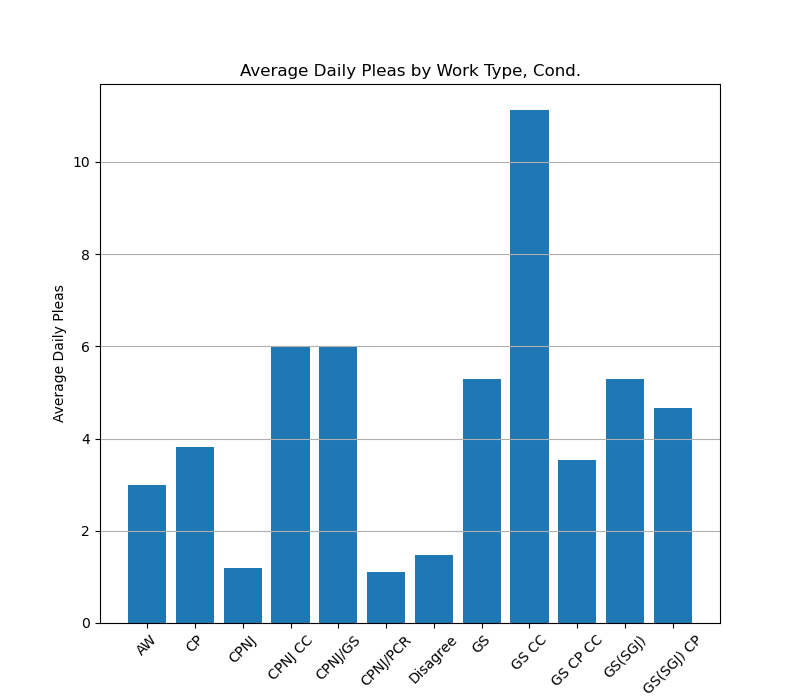
\includegraphics[width=0.75\textwidth, keepaspectratio=true]{../../output/figures/Exploration/avg_pleas_by_worktype_cond.png}
        \end{figure}

      Note that some work types (e.g. GS CC) are fairly uncommon, and are more influenced by outliers. As can be seen from the figure, if we condition on observing a sentencing event, then most of the different work types have roughly similar numbers of pleas processed per day (between 4 and 6). The exceptions to this are CPNJ, CPNJ/PCR, and times where there is a conflict between the sentencing data and the calendar data.

    \paragraph{Days in which we don't observe sentencing events}
      For each assignment type, there are many days in which we don't observe any sentencing events. The next question we had to resolve was which of these days to include. To get a better sense of this, we looked at the average number of pleas processed per day for each work type. Note that this differs from the quantities computed in the previous section because these are not conditional on observing a sentencing event. In other words, this calculation includes days in which we don't observe any sentencing events.

      \begin{figure}[H]
          \centering
          \caption{Snapshot of Judge Calendar}
          \label{fig-cond}
          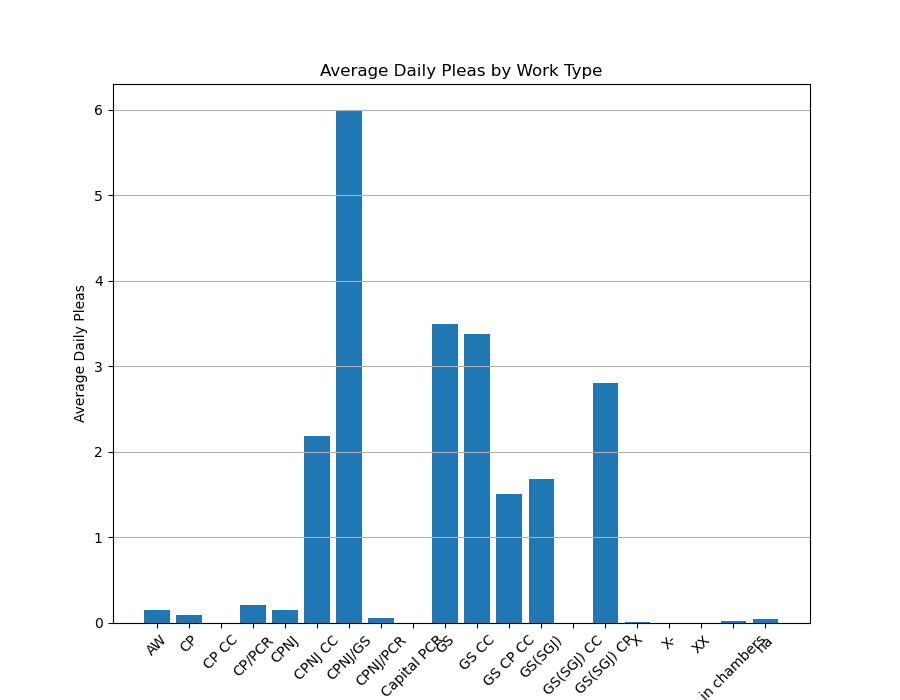
\includegraphics[width=0.75\textwidth, keepaspectratio=true]{../../output/figures/Exploration/avg_pleas_by_worktype.png}
        \end{figure}

      As can be seen from the figure, the average pleas processed per day drops considerably for many work types, especially those that do not include the GS work type. This suggests that for a majority of these days, the judges do not work on criminal cases, and that the days seen in the sentencing data are rare exceptions.

      \paragraph{Decision}
        As previously mentioned, our institutional knowledge suggests that we should count all GS days as criminal days. In addition to this, and following from the previous discussion, we decided to count any day in which we observe a sentencing event as a criminal day as well. For example, if there are 200 GS CC days and we observe sentencing events on 50 of them, we would count those 50 days as 'criminal days'. \textbf{Note/Proposal:} We could include non-GS, but weigh them by their productivity relative to GS days. So for example, if a day of type 'GS CC' sees half the pleas as a GS day, each 'GS CC' day would be counted as half a criminal day.

    \paragraph{Sentencing events with missing dates}
      As previously mentioned, some sentencing events have missing dates. However, they still have information regarding the county and the judge. As a result, we can use the calendar data to narrow down the set of dates in which the sentencing event could have happened. Here, we are assuming that we would only observe a sentencing event for judge $j$ in county $c$ on day $d$ if $j$ was scheduled to be in $c$ on $d$ according to the master calendar. So, for example, if judge 1 has 1 event with a missing date in Aiken county, and he was only assigned to Aiken county on two days according to the master calendar, then the sentencing event must have happened on one of those two days.

      We will deal with trials with missing dates by assigning them as evenly as possible over the days in which the judge was assigned to that county. Suppose judge $j$ has $m$ sentencing events with missing dates in county $c$. We first use the calendar data to determine what days judge $j$ was scheduled to be in county $c$. Let $n_{jc}$ be the number of days that judge $j$ was scheduled to be in county $c$ and let $D_{jc}$ be the set of all days in which judge $j$ was scheduled to be in county $c$. We would assign the missing events to days as evenly as possible, and then assign the remaining days randomly. So, for example, if judge $j$ has 5 events with missing dates in county $c$ and was only scheduled to be in $c$ on two days, then both of those days would get 2 events, and the remaining event would be assigned randomly to one of those two days. \textbf{Question:} Will the set of possible days be those where we already observed sentencing events? Or will it be any day in which the judge was scheduled to be in the county? \textbf{Note:} I think it might be a good idea to restrict $D_{jc}$ and $n_{jc}$ to be the set/number of days in which the judge processed at least one sentencing event, otherwise, we will probably end up with a lot of days with just $1/n_{jc}$ pleas sentenced, which would be excluded from our capacity calculations because we currently exclude days with less than 1 sentencing event. However, this would assume that if a plea is processed at all, it is more likely that it was processed on a day in which other pleas were also processed. We should probably try both ways.

  \subsection{Sample Selection for estimation of $\mu_t$}

\end{document}
